% Общая идея
Параметро-эффективные методы (Parameter-Efficient Fine-Tuning, PEFT) зарекомендовали себя как очень простой и в то же время крайне результативный подход к решению большинства задач.

Общая идея всех методов сводится к:
\begin{enumerate}
    \item использованию больших предобученных языковых моделей (Large Language Models, LLMs);
    \item заморозке всех её параметров;
    \item добавлению небольшого (могут быть десятые доли одного процента от всех параметров) количества дообучаемых параметров;
    \item обучению этих параметров на небольшом наборе данных.
\end{enumerate}

Такой подход даёт следующие преимущества:
\begin{itemize}
    \item если, при наличии набора данных низкого качества, во время классического дообучения (fine-tuning) модель могла ухудшить качество на некоторых задачах, то в этом семействе методов подобного не наблюдается;
    \item значительно снижается необходимое количество размеченных данных – от нескольких сотен до нескольких тысяч примеров;
    \item удобство использования в итоговой системе, потому что достаточно иметь одну большую модель и сколь угодно много адаптеров к ней, которые можно быстро переключать между собой по мере необходимости;
    \item легко дообучать на поступающих новых данных.
\end{itemize}

\subsection{LoRA}
Low-Rank Adaptation of Large Language Models (LoRA) -- метод дообучения, основанный на заморозке весов предобученной модели и добавлении обучаемых матриц ранговой декомпозиции в каждый слой аркитектуры модели, значительно сокращая количество обучаемых параметров \cite{lora}.

Пусть имеется предобученная авторегрессивная языковая модель $P_\Phi(y|x)$, параметризованная $\Phi$.
Каждая задача представлена обучающим набором данных пар контекст-ответ: $\mathcal{Z} = \{(x_i, y_i)\}_{i=1,...,N}$, где оба $x_i$ и $y_i$ представляют собой последовательность токенов.
Во время полноценного дообучения (fine-tuning) модель инициализирована предобученными весами $\Phi_0$ и обновляется как $\Phi_0 + \Delta \Phi$, многократно следуя градиенту для решения максимизационной задачи условного языкового моделирования:
$$
\max_{\Phi}
\sum_{(x,y)\in \mathcal{Z}}
\sum_{t=1}^{|y|}
\log(P_\Phi(y_t|x,y_{<t}))
$$

Основным недостатком является то, что для каждой задачи обучается различный набор параметров $\Delta\Phi$, размерность которого $|\Delta\Phi|$ равна $|\Phi_0|$.
Соответственно, с увеличением размера предобученной модели, хранение и разворачивание множества реплик предобученной модели становится всё более сложной задачей.

В данном подходе применяется более эффективный с точки зрения параметров подход, при котором приращение параметра $\Delta\Phi = \Delta\Phi(\Theta)$ для конкретной задачи дополнительно кодируется набором параметров $\Theta$ гораздо меньшего размера $|\Theta| \ll |\Phi_0|$.
Задача нахождения $\Delta\Phi$ превращается в задачу оптимизации по $\Theta$:
$$
\max_\Theta
\sum_{(x,y)\in \mathcal{Z}}
\sum_{t=1}^{|y|}
\log(p_{\Phi_0 + \Delta\Phi(\Theta)}(y_t|x,y_{<t}))
$$

Нейронная сеть состоит из множества полносвязных слоёв, которые выполняют матричное перемножение.
Матрицы весов в этих слоях обычно являются полноранговыми.
Исследования показывают, что при адаптации к специфической задаче предобученные подели имеют маленькую "`внутреннюю размерность"' и могут эффективно обучаться, несмотря на случайную проекцию в меньшее подпространство \cite{aghajanyan2020intrinsic}.
Из данного наблюдения вытекает гипотеза, что обновления веса моделей тоже имеют небольшую "`внутреннюю размерность"'.
Для предобученной матрицы весов $W_0 \in \mathbb{R}^{d \times k}$ ограничивается её обновления, представляя его в виде разложения низкого ранга $W_0+\Delta W = W_0 + BA$, где $B \in \mathbb{R}^{d \times k}, A\in \mathbb{R}^{r \times k}$ и ранг $r \ll min(d,k)$.
Во время обучения матрица $W_0$ заморожена и не получает обновлений от градиента, в то время как $A$ и $B$ являются обучаемыми параметрами.
Оба $W_0$ и $\Delta W = BA$ умножаются на одинаковый вектор, а их соответствующие выходные вектора по-координатно суммируются.
Для $h = W_0 x$ модифицированный прямой проход:
$$h = W_0x + \Delta W x = W_0x + BAx$$
Данное выражение изображено на рисунке \ref{fig:lora}.
Для $A$ используется случайная Гауссова инициализация, а $B$ инициализируется нулями, так что $\Delta W = BA$ равна нуля в начале обучения.

\begin{figure}[ht]
  \centering
  \frame{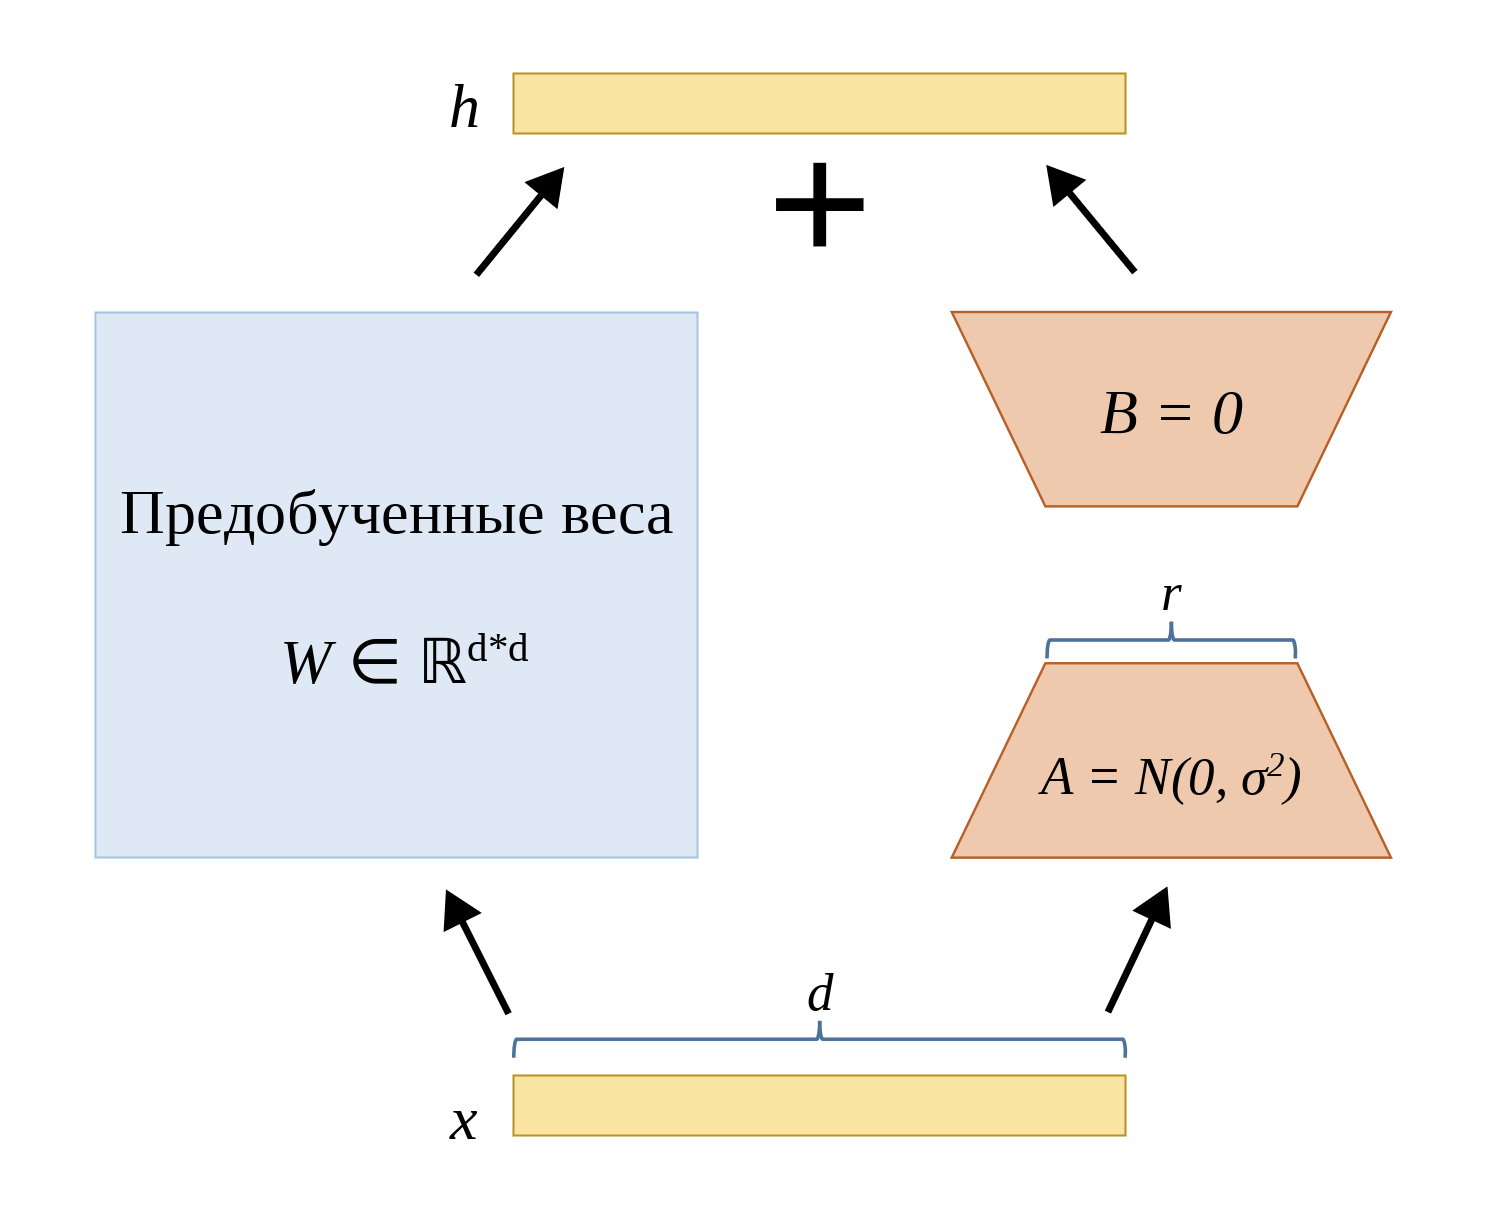
\includegraphics[width=0.7\textwidth]{figures/lora.png}}
  \caption{Параметризация весов в алгоритме LoRA. Обновляются только матрицы $A$ и $B$}
  \label{fig:lora}
\end{figure}

В работе с помощью данного алгоритма была дообучена модель \texttt{cointegrated/rut5-base-paraphraser} на собранном наборе данных.
Метрики качества указаны в таблице \ref{table:results}, а примеры генерации в  в приложении \ref{cha:appendix1}.


\subsection{P-Tuning}
Данный метод основан на автоматическом поиске затравок (prompts) в непрерывном пространства \cite{gpt_understands_too}.

Пусть дана предобученная языковая модель $\mathcal{M}$.
Последовательность дискретных входных токенов 
$x_{1:n} = \{x_0, x_1, ..., x_n\}$
будет сопоставлена с входными эмбеддингами 
$\{\mathbf{e}(x_o), \mathbf{e}(x_1), ..., \mathbf{e}(x_n)\}$
с помощью предварительно обученного слоя ембеддингов
$\mathbf{e} \in \mathcal{M}$.
В конкретном случае, зависящем от контекста $\mathbf{x}$, часто используются выходные эмбеддинги набора целевых токенов  $\mathbf{y}$ для последующей обработки.

Функция затравки (промпта) $\mathbf{p}$ - организовать контекст $\mathbf{x}$, результат $\mathbf{y}$ и саму себя в шаблон $T$.
Для задачи переноса стиля текста шаблоном может быть "<Перепиши предложение "`$\mathbf{x}$"' в неформальном стиле: "`$\mathbf{y}$"'">.
Здесь "<Перепиши предложение ... в неформальном стиле: ..."> это затравка, $\mathbf{x}$ это контекст, а $\mathbf{y}$ это результат.

Пусть $\mathcal{V}$ это словарный запас языковой модели $\mathcal{M}$, а $[P_i]$ является $i$-ым токеном шаблона $T$.

Имея шаблон $T = \{ [P_{0:i}],x,[P_{i+1:m}], y \}$, дискретная затравка удовлетворяет условию $[P_i] \in \mathcal{V}$ и превращает $T$ в
$$\{ \mathbf{e}([P_{0:i}]), \mathbf{e}(\mathbf{x}), \mathbf{e}([P_{i+1:m}]),\mathbf{e}(\mathbf{y}) \}$$

В отличии от этого, P-tuning воспринимает $[P_i]$ как псевдо-токены и превращает шаблон в
$$\{h_0, ..., h_i, \mathbf{e}(\mathbf{x}), h_{i_1}, ..., h_m, \mathbf{e}(\mathbf{x})\}$$
где $h_i(0 \leqslant i < m)$ это обучаемые эмбеддинги.
Это позволяет находить лучшие непрерывные затравки вне словарного запаса, которым оперирует языковая модель.
Сравнение дискретного поиска и P-tuning приллюстрировано на рисунке \ref{fig:p_tuning}.

Имея функцию потерь $\mathcal{L}$ можно дифференциально оптимизировать непрерывные затравки $h_i(0 \leqslant i < m)$ как
$$\hat{h}_{0:m} = \arg\min_h \mathcal{L} (\mathcal{M}(\mathbf{x},\mathbf{y}))$$

\begin{figure}[ht]
  \centering
  \frame{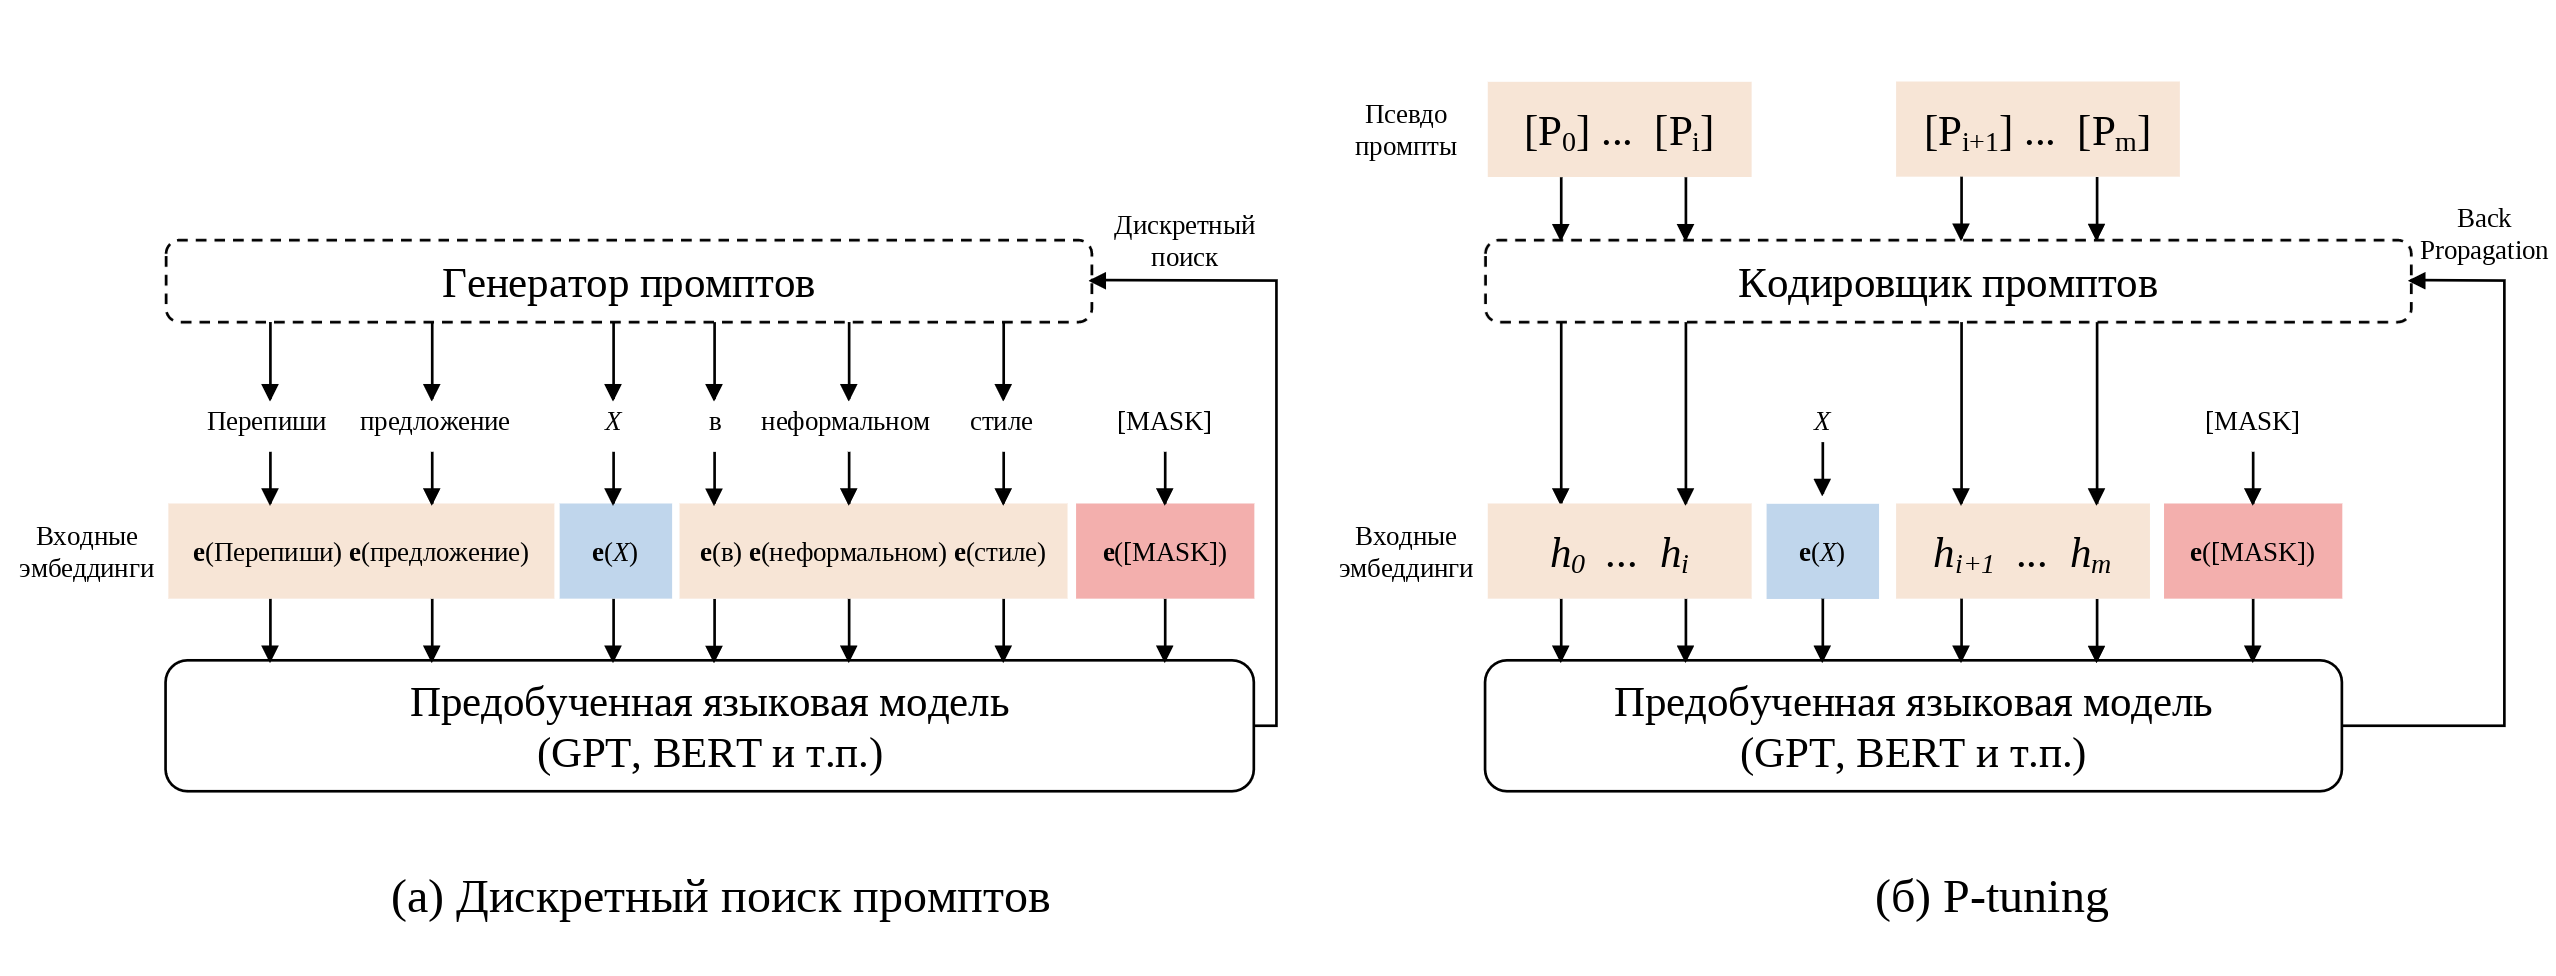
\includegraphics[width=1.0\textwidth]{figures/p_tuning.png}}
  \caption{P-tuning}
  \label{fig:p_tuning}
\end{figure}

В работе с помощью данного алгоритма была дообучена модель \texttt{ai-forever/rugpt3small\_based\_on\_gpt2} на собранном наборе данных.
Метрики качества указаны в таблице \ref{table:results}, а примеры генерации в  в приложении \ref{cha:appendix1}.